%% Based on a TeXnicCenter-Template by Gyorgy SZEIDL.
%%%%%%%%%%%%%%%%%%%%%%%%%%%%%%%%%%%%%%%%%%%%%%%%%%%%%%%%%%%%%

%------------------------------------------------------------
%
\documentclass[a4paper,12pt]{letter}%
%Options -- Point size:  10pt (default), 11pt, 12pt
%        -- Paper size:  letterpaper (default), a4paper, a5paper
%        -- Orientation  (portrait is the default)
%                        landscape
%        -- Print size:  oneside (default), twoside
%        -- Quality      final(default), draft
%        -- Title page   notitlepage(default)
%        -- Columns      onecolumn(default)
%        -- Equation numbering (equation numbers on the right is the default)
%                        leqno
%        -- Displayed equations (centered is the default)
%                        fleqn (equations start at the same distance from the
%                        right side)
%        -- Open bibliography style (closed is the default)
% For instance the command
%           \documentclass[a4paper,12pt,leqno]{letter}
% ensures that the paper size is a4, the fonts are typeset at the size 12p
% and the equation numbers are on the left side
%
\usepackage{amsmath}%
\usepackage{amsfonts}%
\usepackage{amssymb}%
\usepackage{graphicx}
%
\usepackage{t1enc}
\usepackage[latin2]{inputenc}
%---- Setting the margins
%
\setlength{\textwidth}{160mm}%
\setlength{\hoffset}{-0.4mm}%
\setlength{\oddsidemargin}{0mm}%
\setlength{\topskip}{0mm}%
\setlength{\textheight}{240mm}%
\setlength{\topmargin}{0mm}%
\setlength{\voffset}{-5.4mm}
%
%-------------------------------------------------------------
%
\name{Bibliograf\'ia}%
\address{Instituto Polit\'ecnico Nacional\\
         Escuela Superior de C\'omputo\\
         Grupo 2CM4\\
         Teor\'ia Computacional\\
				Nava Vivas Ana Paola\\
				\hrulefill}

%-------------------------------------------------------------
\begin{document}
\begin{letter}%
{Jerarqu\'ia de Chomsky\\
}
\opening{}


La jerarqu\'ia de Chomsky consta de cuatro niveles:
\begin{center}
\begin{figure}
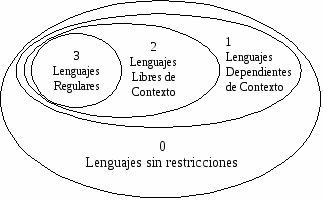
\includegraphics[width=0.9\textwidth]{Jerarquia_Chomsky.png} 
\centering
\end{figure}
\end{center}
\begin{enumerate}
  \item Gram\'aticas de tipo 0: no tienen restricciones y son recursivas, incluye a todas las gram\'aticas formales. Estas gram\'aticas generan todos los lenguajes capaces de ser reconocidos por una m\'aquina de Turing. Los lenguajes son conocidos como lenguajes recursivamente enumerables. N\'otese que esta categor\'ia es diferente de la de los lenguajes recursivos, cuya decisi\'on puede ser realizada por una m\'aquina de Turing que se detenga.

  \item Gram\'aticas de tipo 1 (dependientes de contexto):
Generan los lenguajes dependientes de contexto. Contienen reglas de producci\'on de la forma:

\begin{center}
\begin{figure}
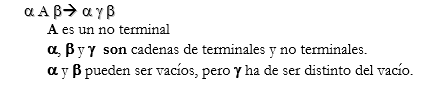
\includegraphics[width=0.9\textwidth]{tipo1.png} 
\centering
\end{figure}
\end{center}

\begin{lstlisting}

Se denominan gram\'aticas dependientes del contexto, porque, como se observa, A puede ser sustituido por $\gamma$ si est\'a acompa\~nada de $\alpha$ por la izquierda y de $\beta$ por la derecha.  
Estos lenguajes son todos los lenguajes que pueden ser reconocidos por una m\'aquina de Turing no determinista.

\end{lstlisting}


  \item Gram\'aticas Tipo 2 (independientes de contexto):
Generan los lenguajes libres de contexto. Est\'an definidas por  reglas de la forma:
\begin{center}
\begin{figure}
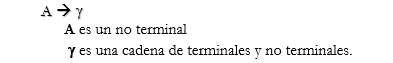
\includegraphics[width=0.9\textwidth]{tipo2.png} 
\centering
\end{figure}
\end{center}

Se denominan independientes de contexto porque A puede sustituirse por $\gamma$ independientemente de las cadenas por las que est\'e acompa\~nada. 
Los lenguajes independientes  de contexto constituyen la base te\'orica para la sintaxis de la mayor\'ia de los lenguajes de programaci\'on. Definen la sintaxis de las declaraciones, las proposiciones, las expresiones, etc.(es decir, la estructura de un programa)

  \item Gram\'aticas Tipo 3 (gram\'aticas regulares):
Generan los lenguajes regulares. Las reglas se restringen a un \'unico no terminal en la parte izquierda y una parte derecha compuesta por un \'unico terminal que puede estar seguido o no de un \'unico no terminal. Es decir, normas del tipo: 
\begin{center}
\begin{figure}
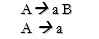
\includegraphics[width=0.3\textwidth]{tipo3.png} 
\centering
\end{figure}
\end{center}
Estos lenguajes son los que pueden ser decididos por un aut\'omata finito (regular). Los lenguajes regulares se utilizan para definir estructura l\'exica de los lenguajes de programaci\'on. Definen la sintaxis de los identificadores, n\'umero, cadenas y otros s\'imbolos b\'asicos del lenguaje. 


\end{enumerate}

\begin{center}
\begin{figure}
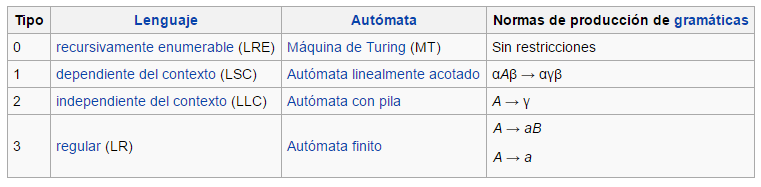
\includegraphics[width=1\textwidth]{malditajerarquia.png} 
\centering
\end{figure}
\end{center}

\begin{lstlisting}

\end{lstlisting}
\begin{lstlisting}

\end{lstlisting}
\begin{lstlisting}

\end{lstlisting}
\begin{lstlisting}

\end{lstlisting}
\begin{lstlisting}

\end{lstlisting}
\begin{lstlisting}
.

.

.

.
\end{lstlisting}

.
\closing{   } \vspace{5mm}%
\begin{center}
\begin{figure}
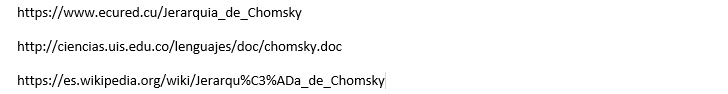
\includegraphics[width=0.9\textwidth]{tochebibliografia.png} 
\centering
\end{figure}
\end{center}

\end{letter}
\end{document}
